\section{Mathematical background}
\label{sec:math}

% Singular Value Decomposition in general

Singular value decomposition \cite{Baker2005, Kalman1996, Golub1996} is based on a theorem from linear algebra which says that a rectangular matrix $\mtrx{A} \in \mathbb{R}^{m \times n}$ can be decomposed into the product of three matrices - an orthogonal matrix $\mtrx{U} \in \mathbb{R}^{m \times m}$, a diagonal
matrix $\mtrx{S} \in \mathbb{R}^{m \times n}$, and the transpose of an orthogonal matrix $\mtrx{V} \in \mathbb{R}^{n \times n}$:

\begin{equation}
\mtrx{A} = \mtrx{U} \mtrx{S} \mtrx{V}^\mathsf{T},
\label{eq:svd-def}
\end{equation}

\noindent
where $\mtrx{U^\mathsf{T}U} = \mtrx{I}$, $\mtrx{V^\mathsf{T}V} = \mtrx{I}$. The columns of $\mtrx{U}$ are orthonormal eigenvectors of $\mtrx{AA^\mathsf{T}}$, which are called the left singular vectors. The columns of $\mtrx{V}$ are orthonormal eigenvectors of $\mtrx{A^\mathsf{T}A}$ called the right singular vectors. $\mtrx{S}$ (sometimes referred to as $\mtrx{\Sigma}$) is a diagonal matrix containing singular values in descending order, which are at the same time the nonzero square roots of the eigenvalues of $\mtrx{AA^\mathsf{T}}$ and $\mtrx{A^\mathsf{T}A}$.

% The singular values are the nonzero square roots of the eigenvalues from AAT and ATA. The eigenvectors of AAT are called the \left" singular vectors (U) while the eigenvectors of ATA are the right" singular vectors (V).

SVD can be seen as a method for transforming correlated variables into a set of uncorrelated ones. At the same time, SVD is a method for ordering the dimensions based on variation and identifying the dimension with the largest variation. Once this dimension is identified, it is possible to find the best approximation of the original data points using fewer dimensions. Hence, SVD can be seen as a method for data reduction/compression.

\subsection{SVD compression}

This is the basic idea behind SVD: taking a high dimensional, highly variable set of data points and reducing it to a lower dimensional space that exposes the substructure of the original data more clearly and orders it from the largest variation to the least. What makes SVD practical for data compression applications is that variation below a particular threshold can be simply ignored to massively reduce data with assurance that the main relationships of interest have been preserved.

The objective of a compression algorithm is to reduce amount of data representing FEM results and also the ability to reconstruct original data from its smaller representation. This saves storage capacity and also accelerates the data transfer between computers as the analysis itself and the post-processing of results is sometimes done on different workstations.

A compression method can be lossy or lossless. Lossless methods are able to fully reconstruct original data. Lossy methods, on the other hand, produce only approximations of original data.

SVD is used in this paper as a part of the compression algorithm. The SVD method applied to arbitrary matrix produces decomposition that consists of corresponding singular values and singular vectors. This process is fully reversible (with the assumption that the numerical errors are negligible). The original matrix can be reconstructed by the multiplication of decomposed parts. However, the compression algorithm is based on modification of decomposition to create low-rank approximation matrix. The reconstructed matrix slightly differs from the original matrix and algorithm therefore performs lossy compression.

\subsection{Low-rank approximation matrix}

From the definition of SVD in (\ref{eq:svd-def}) and from the properties of SVD, the fact follows that a matrix can be represented in the form of its SVD components as a sum of $n$ rank-1 matrices

\begin{equation}
\mtrx{A}=\sum_{i=1}^{n} s_{i}\mathbf{u}_{i}\mathbf{v}_{i}^{\mathsf{T}},
\label{eq:svd-expansion}
\end{equation}

\noindent
where $s_i$ is the $i$-th singular value, $\mathbf{u}_i$ and $\mathbf{v}_i$ are corresponding singular vectors, and $n$ is the rank of matrix~$\mtrx{A}$. Considering the fact that singular values are ordered $s_{1} \geq s_{2} \geq s_{3} \geq ... \geq s_{n}$, the above formula implies that the first term of the sum would have the highest contribution and the last term would have the lowest contribution to matrix~$\mtrx{A}$. Therefore, if we take only first $r$ members of the above summation we get an approximation matrix

\begin{equation}
\mtrx{A'}=\sum_{i=1}^{r} s_{i}\mathbf{u}_{i}\mathbf{v}_{i}^{\mathsf{T}}.
\label{eq:svd-approx-expansion}
\end{equation}

Quality of approximation depends on the magnitude of the singular values omitted from the approximation formula, namely $s_{r+1} ...  s_{n}$. The compression algorithm is based on an assumption that the first singular value is order-of-magnitude higher than singular values at the end of the decomposition sequence. In special cases, when $r=n$, or $s_{i}=0$ for all $i > r$, the omitted singular values do not contribute to the sum and the compression is therefore lossless. In other cases, approximation error has to be calculated and taken into account to avoid loss of important details in data.

The main goal of the compression algorithm is to find a compromise between low approximation error and high compression ratio $c$ which is calculated using the formula

\begin{equation}
c=\frac{r(m+n+1)}{m n},
\label{eq:cr-def}
\end{equation}

\noindent
where $m$ and $n$ are dimensions of matrix $\mtrx{A}$. Explanation of the compression ratio formula is best done using Figure~\ref{fig:lowrank_svd}. Light color represents the part of matrix decomposition that is to be stored in the output file as a low-rank approximation of the input.

\begin{figure}[H]
\centering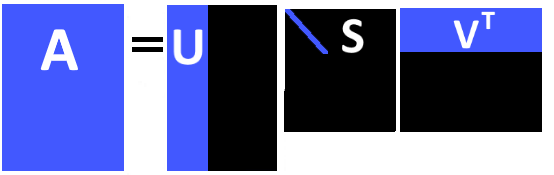
\includegraphics[width=0.7\textwidth]{figures/low_rank_decomposition_diagram}
\caption{Decomposition of input matrix $\mtrx{A}$ into diagonal matrix of singular values $\mtrx{S}$ and matrices of left and right singular vectors. Light color illustrates low-rank approximation.}
\label{fig:lowrank_svd}
\end{figure}

\subsection{Error estimation}
\label{sec:error}

Low-rank approximation matrix method that is described in this paper is a lossy compression technique. Several error metrics are used to control the quality of results \cite{SairaBanu2015}.

\begin{itemize}

\item \textbf{Mean Square Error}
\begin{equation}
\mathit{MSE}=\frac{1}{m n} \sum_{i=1}^{m} \sum_{j=1}^{n} (a_{ij} - a'_{ij})^{2},
\label{eq:mse-def}
\end{equation}

\noindent
where $a_{ij}$ represents an element of the original matrix and $a'_{ij}$ represents an element of the
reconstructed matrix of dimension $m \times n$.

\item \textbf{Rooted Mean Square Deviation}
\begin{equation}
\mathit{RMSD} = \sqrt{\mathit{MSE}}.
\label{eq:rmsd-def}
\end{equation}

\item \textbf{Normalized Rooted Mean Square Deviation}
\begin{equation}
\mathit{NRMSD} = \frac{\mathit{RMSD}}{X_{max}-X_{min}}=\frac{\sqrt{\mathit{MSE}}}{X_{max}-X_{min}},
\label{eq:nrmsd-def}
\end{equation}

\noindent
where $X_{min}$ and $X_{max}$ are elements of input matrix $\mtrx{A}$ with minimum and maximum value, respectively. This error metric is able to measure and compare errors in datasets with different scales. Therefore, it is the main parameter that is used to control the quality of compression in the algorithm presented in this paper.

\item \textbf{Peak Signal to Noise Ratio}

$\mathit{PSNR}$ is most commonly used to measure the quality of reconstruction of lossy compression methods (e.g. image compression). The signal in this case is the original data, and the noise is the error introduced by compression. $\mathit{PSNR}$ is an approximation to human perception of reconstruction quality. This metric is not so important in area of FEM analyses, where the human perception of visualizations is not as important as the exact mathematical accuracy of approximations. The reason to include $\mathit{PSNR}$ in results is in particular to allow comparison with other image-related compression methods. $\mathit{PSNR}$ is usually expressed in terms of the logarithmic decibel scale (dB)

\begin{eqnarray}
\mathit{PSNR} &=& 10\log_{10}\frac{(X_{max}-X_{min})^{2}}{\mathit{MSE}} =
\\
&=& 20\log_{10}\frac{X_{max}-X_{min}}{\sqrt{\mathit{MSE}}}=20\log_{10}\frac{1}{\mathit{NRMSD}} = \nonumber
\\
&=& -20\log_{10}\mathit{NRMSD}. \nonumber
\label{eq:psnr-def}
\end{eqnarray}

\item \textbf{Normalized Maximum Error}
\begin{equation}
\mathit{NME} = \frac{\lVert \mtrx{A} - \mtrx{A'} \lVert_{\max}}{X_{max}-X_{min}} = \frac{\max\limits_{ij}(a_{ij} - a'_{ij})}{X_{max}-X_{min}}.
\label{eq:nme-def}
\end{equation}

\end{itemize}

\subsection{Randomized SVD}

The exact SVD of a $m \times n$ matrix has computational complexity \newline $\mathrm{O}(\mathrm{min}(mn^2, m^2n))$ using the "big-O" notation. When applied on large data sets it tends to be very time-consuming. In \cite{Candes2011, Woolfe2008, Martinsson2011, Szlam2014}, there are described randomized methods for constructing approximate matrix factorizations which offer significant speedups over classical methods.

The particular implementation of the randomized decomposition is based on the algorithm described in \cite{Halko2011}. The authors proposed an algorithm for efficient computation of low-rank approximation to a given matrix. The algorithm can be split into two main computational stages.

The first stage is to construct a low-dimensional subspace that captures the action of the matrix. To be more formal, this stage is to compute an approximate basis for the range of the input matrix $\mtrx{A}$. This basis matrix $\mtrx{Q}$ is required to have orthonormal columns and

\begin{equation}
\mtrx{A} \approx \mtrx{Q} \mtrx{Q}^{\mathsf{T}} \mtrx{A}.
\end{equation}

\noindent
Matrix $\mtrx{Q}$ is desired to contain as few columns as possible while producing accurate approximation of matrix $\mtrx{A}$ at the same time.

The second stage is to use $\mtrx{Q}$ to obtain approximate SVD factorization of $\mtrx{A}$. This can be achieved using simple deterministic steps:

\begin{enumerate}
\item Construct $\mtrx{B} = \mtrx{Q}^{\mathsf{T}} \mtrx{A}$.
\item Compute an exact SVD of the small matrix: $\mtrx{B}=\mtrx{W}\mtrx{\widetilde{S}}\mtrx{\widetilde{V}}^{\mathsf{T}}$.
\item Set $\mtrx{\widetilde{U}}=\mtrx{Q}\mtrx{W}$.
\end{enumerate}

The main challenge is therefore to efficiently construct $r$ orthonormal vectors forming the matrix $\mtrx{Q}$ that (nearly) span the range of $\mtrx{A}$; $r$ is the desired rank of approximation and is supposed to be substantially less then both dimensions of $\mtrx{A}$. After that an SVD that closely approximates $\mtrx{A}$ can be constructed (closely in the sense that the spectral norm of the difference between $\mtrx{A}$ and the approximation to $\mtrx{A}$ is small relative to the spectral norm of $\mtrx{A}$).

In order to estimate the range of matrix $\mtrx{A}$, it is applied to a collection of $r$ random vectors. The result of applying $\mtrx{A}$ to any vector is a vector in the range of $\mtrx{A}$, and if the matrix is applied to $r$ random vectors, the results will nearly span the range of $\mtrx{A}$ with extremely high probability. Mathematical proofs given in \cite{Halko2011} and \cite{Witten2015} show that the probability of missing a substantial part of the range of $\mtrx{A}$ is negligible if the vectors to which we apply $\mtrx{A}$ are sufficiently random (i.e. entries of these vectors are independent and identically distributed).

Therefore, the matrix $\mtrx{A}$ is applied to a random Gaussian matrix $\mtrx{\Omega}$ that contains $r$ columns with random normally distributed entries yielding the matrix $\mtrx{Y} = \mtrx{A} \mtrx{\Omega}$. Applying the Gram-Schmidt process (or any other method for constructing QR decomposition) produces the decomposition $\mtrx{Y}=\mtrx{Q}\mtrx{R}$, where columns of $\mtrx{Q}$ are an orthonormal basis for the range of $\mtrx{Y}$, and since columns of $\mtrx{Y}$ nearly span the range of $\mtrx{A}$, $\mtrx{Q}$ is an orthonormal basis for the approximate range of $\mtrx{A}$.

$\mtrx{A}$ is then decomposed as
\begin{equation}
\mtrx{A} \approx \mtrx{Q}\mtrx{Q}^{\mathsf{T}}\mtrx{A} = \mtrx{Q}\mtrx{B} = \mtrx{Q}\mtrx{W}\mtrx{\widetilde{S}}\mtrx{\widetilde{V}}^{\mathsf{T}} = \mtrx{\widetilde{U}}\mtrx{\widetilde{S}}\mtrx{\widetilde{V}}^{\mathsf{T}}.
\end{equation}

\noindent
The algorithm produces matrices $\mtrx{\widetilde{U}}$ and $\mtrx{\widetilde{V}}$ with orthonormal columns being approximations of the left and the right singular vectors of matrix $\mtrx{A}$, and a nonnegative diagonal matrix $\mtrx{\widetilde{S}}$ that contains approximations of the first $r$ singular values of matrix $\mtrx{A}$. For a dense input matrix, randomized SVD algorithm requires $\mathrm{O}(mn \log{r})$ floating-point operations, substantially less than classical algorithms.
